\section{Multi-Agent World}
\label{sec:method}

As shown in Figure~\ref{fig:overview}, MAW develops multi-agent orchestration in two stages that share one construction record.
The first stage turns existing single-agent backends into multi-agent environments, in which a task carries subtasks that several agents can execute simultaneously.
The second stage trains an orchestrator inside those environments under a reward that reads how the agent team actually distributed the work.


\begin{figure}[t]
  \centering
  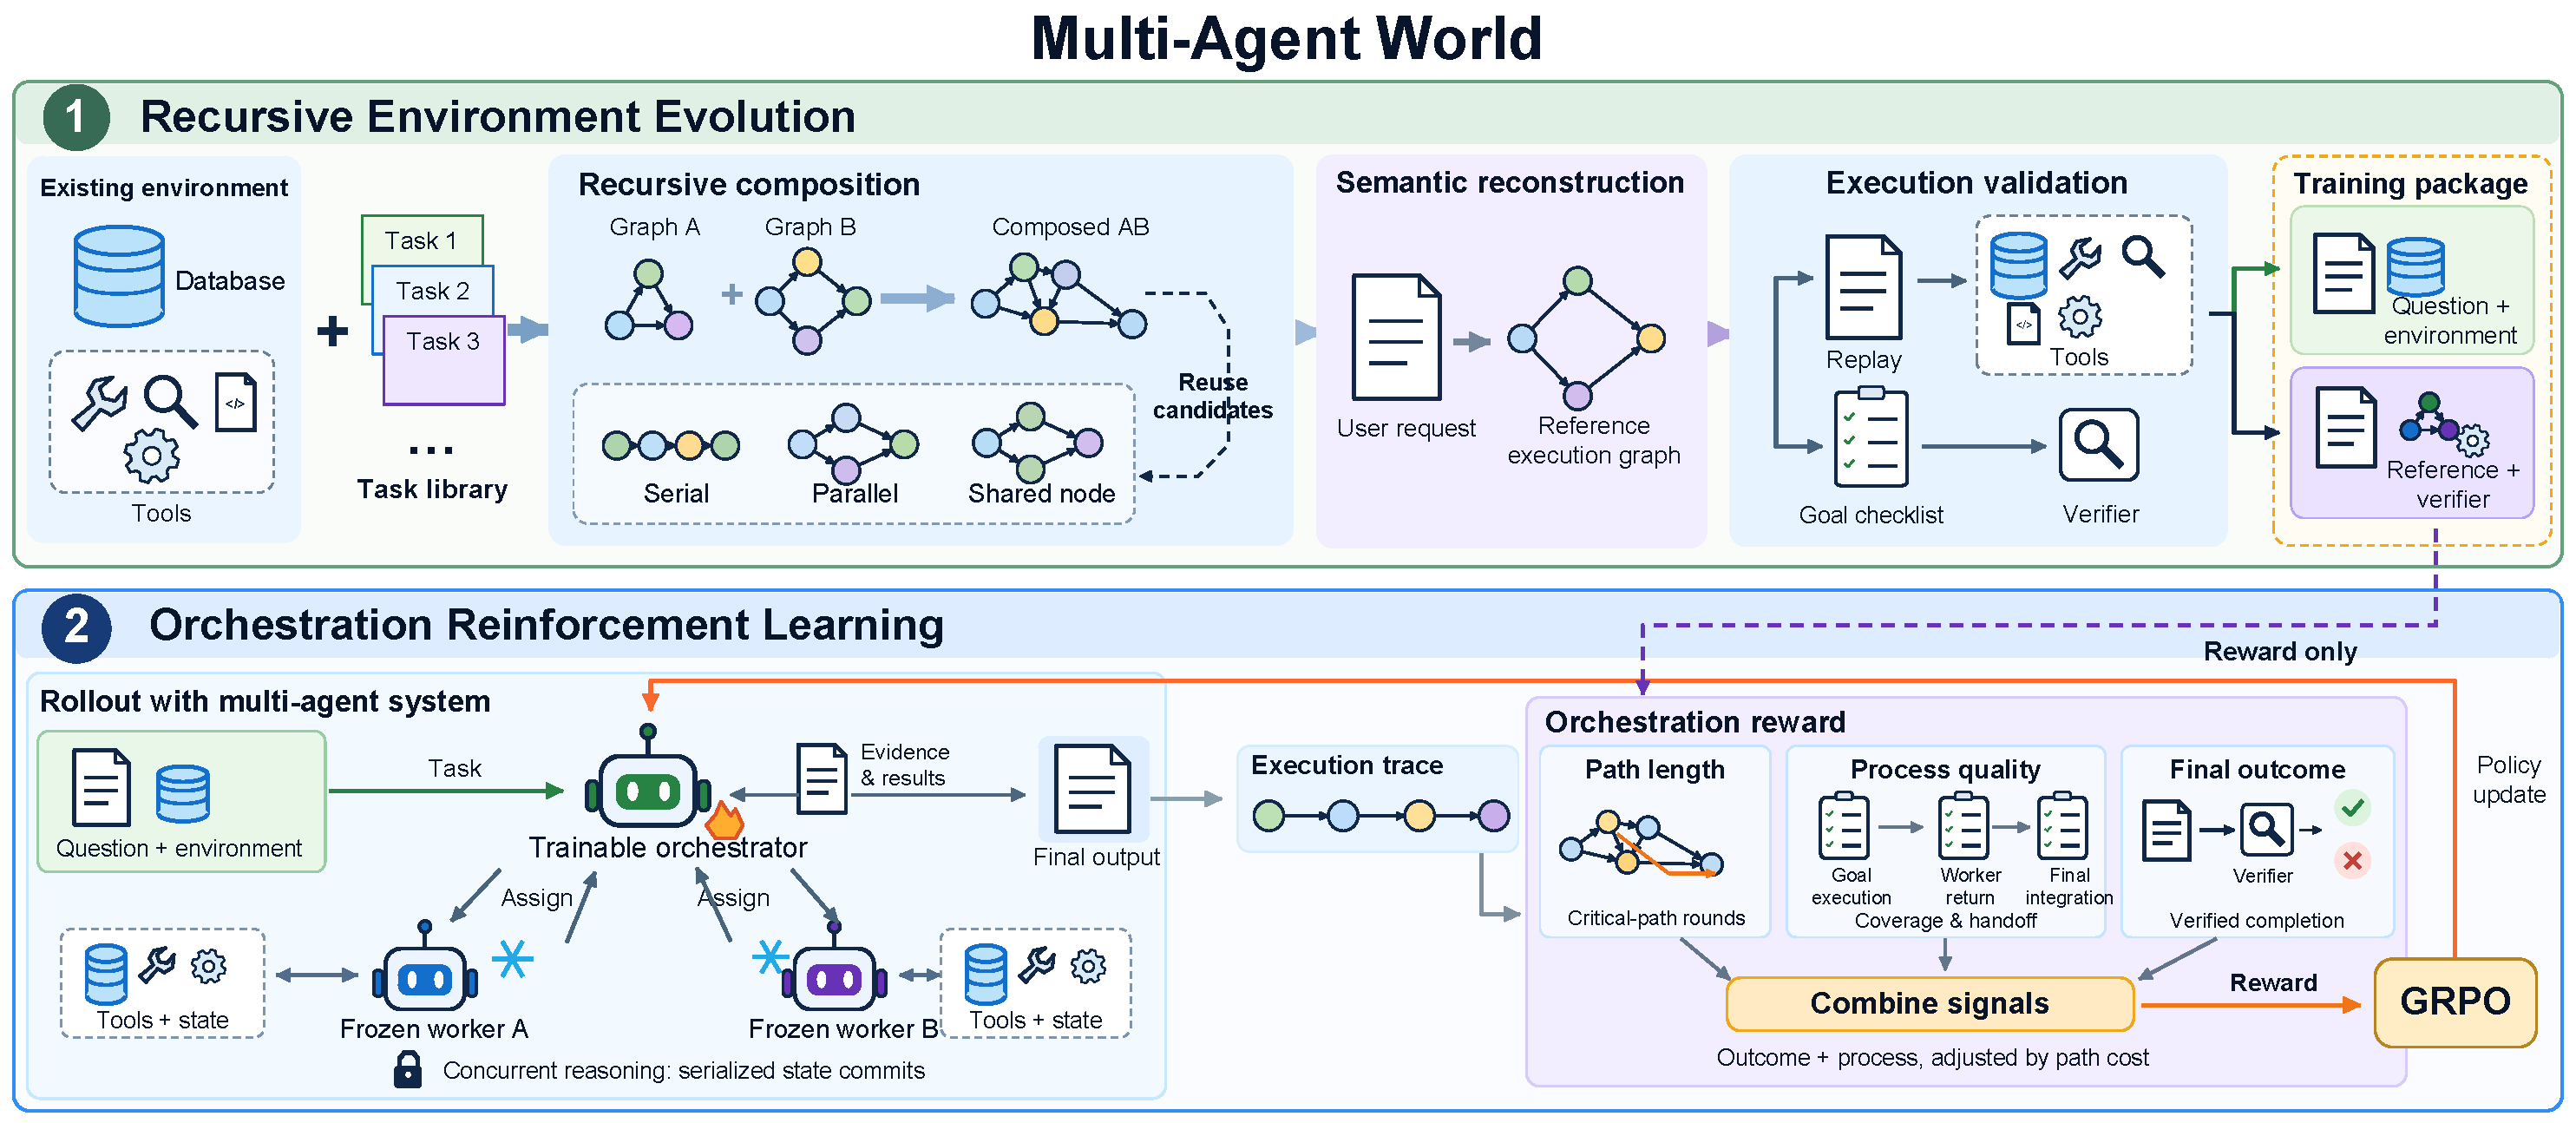
\includegraphics[width=0.99\linewidth]{figures/figure2.pdf}
  \caption{Overview of MAW. Recursive environment improvement composes the reference graphs of existing tasks, reconstructs each composed graph into one request, and admits it only after replay and verification. The resulting package supplies the interactive environment to the agent team and the hidden reference to the reward service, and only the orchestrator is updated.}
  \label{fig:overview}
\end{figure}

\subsection{From Single-Agent to Multi-Agent Environments}
\label{sec:ma-env}

An agentic environment is written as $\mathcal{E}=(\mathcal{S},\mathcal{U},f_{\mathrm{exec}},s_0)$, where $\mathcal{S}$ is a database-backed state space, $\mathcal{U}$ is the tool interface, and $s_0$ is the initial state.
The transition $f_{\mathrm{exec}}(s,u)=(s',o)$ executes a tool call $u$ and returns an observation $o$.
Following the synthesis setting of AWM and Agent-World~\citep{wang2026agentworldmodelinfinity,dong2026agentworld}, a task in $\mathcal{E}$ is written as $x=(q,G,a^{\star},\Delta^{\star})$.
Here $q$ is the user request, $a^{\star}$ is the reference answer, and $\Delta^{\star}$ is the required change of the database.
The reference task graph $G=(V,A)$ has one node $v\in V$ per reference tool call, and an edge $(u,v)\in A$ means that $v$ consumes an output or a state effect of $u$.

A multi-agent environment extends this setting with a delegation interface and an independence record.
The interface $\mathcal{H}$ lets an orchestrator create workers and assign subtasks to them, which is what makes a team executable at all.
The record $\Pi$ closes the supervision gap of Section~\ref{sec:intro}, since it names the branches against which a schedule can be scored, while the structural gap is closed by the composition that creates those branches.
We write a multi-agent environment as $\mathcal{E}^{\mathrm{ma}}=(\mathcal{S},\mathcal{U},f_{\mathrm{exec}},s_0,\mathcal{H})$ and a multi-agent task as $x^{\mathrm{ma}}=(q,G,a^{\star},\Delta^{\star},\Pi)$.
Here $\Pi\subseteq V\times V$ contains the pairs of reference calls that are verified to be executable in either order.
Orchestration training consumes this record, without which a verifier reports only whether the team produced the correct answer and leaves the correctness of a simultaneous execution unmeasured.
Existing pipelines produce $(q,G,a^{\star},\Delta^{\star})$ for one agent and leave $\Pi$ empty, which is why their tasks train tool use and not orchestration.

\subsection{Recursive Environment Improvement}
\label{sec:synthesis}

In this stage, we aim to turn existing single-agent backends into multi-agent environments without building new ones from scratch, which is challenging as branch structure cannot be requested from a generator directly.
When a model is asked for a parallel task, it tends to produce two unrelated questions in one prompt, leaving an executable reference that is either trivial or inconsistent.
MAW instead constructs branch structure at the level of reference graphs, where independence is a checkable property, and writes the graph as natural language only afterwards.

\textbf{Recursive Composition.}\quad
Before any natural language is generated, composition introduces a controlled amount of dependency and independence into a task.
From a seed pool $\mathcal{C}$ of single-agent tasks in the same backend, MAW composes two of them into a candidate graph,
\begin{equation}
\tilde{G}=f_{\mathrm{comp}}^{z}(G_1,G_2),\qquad z\in\{\mathrm{serial},\mathrm{parallel}\},
\label{eq:compose}
\end{equation}
where the serial operator adds an edge between a pair $(v_1,v_2)\in V_1\times V_2$ whose output or state effect fills an argument of the other.
In contrast, the parallel operator takes the disjoint union with no edge between the two sides and lets one answer node consume both.
After composition, a candidate graph re-enters $\mathcal{C}$ and acquires further subtasks in later rounds, so mixed structure arises from repeated application.
For each edge, MAW stores the operator that produced it, which later distinguishes a branch from an accidental ordering, and Appendix~\ref{app:synthesis} gives a worked example of two rounds.


\textbf{Semantic Reconstruction.}\quad
A composed graph is not yet a request a user would write, as the two parents may refer to different entities or reporting formats.
Reconstruction produces one coherent request and an executable reference plan, written as $(q,G)=f_{\mathrm{recon}}(\tilde{G},q_1,q_2,\mathcal{U})$, during which MAW aligns entities across the two sides, merges reads that return the same content, and inserts a lookup when the combined goal needs one.
The request states the desired outcome and exposes neither the reference plan nor any hint about how many workers to use, thereby leaving the decomposition to the policy.

\textbf{Execution-grounded Admission.}\quad
As repeated composition can accumulate redundant calls or combine requirements that no single execution satisfies, MAW admits a task only when its reference survives execution and inspection.
Executing the plan from a reset state gives $(a^{\star},\Delta^{\star})=f_{\mathrm{exec}}^{\ast}(G,s_0)$, and MAW then replays it from a fresh state.
MAW admits a task only when execution, replay, and an independent review all pass, written as $f_{\mathrm{gate}}=f_{\mathrm{run}}\cdot f_{\mathrm{replay}}\cdot f_{\mathrm{sem}}\in\{0,1\}$ and specified in Appendix~\ref{app:synthesis}.
Admission is the step that keeps a composed candidate from entering training as an unsolvable or self-contradictory task.

\textbf{Verified Independence Record.}\quad
Although composition proposes that two subtasks lie on separate branches, the proposal is not yet verified, as reconstruction may introduce a shared entity that makes one side depend on the other.
MAW verifies every proposed branch by execution before recording it,
\begin{equation}
\Pi=\bigl\{(v,v')\in V_{\mathrm{r}}\times V_{\mathrm{r}} \,:\, v\nprec v',\; v'\nprec v,\; f_{\mathrm{perm}}(v,v')=1\bigr\},
\label{eq:pi}
\end{equation}
where $V_{\mathrm{r}}\subseteq V$ is the set of read-only calls and $v\prec v'$ denotes that $v'$ is reachable from $v$ in $G$.
The test $f_{\mathrm{perm}}(v,v')$ executes the reference plan again with the order of the two calls exchanged, returning one when the answer and the database effect are unchanged.
Together with its resettable environment, its checker, and its hidden reference, this record converts a synthesized task into a multi-agent task.
One construction therefore produces two things at once, namely the branches an orchestrator can act on and the ground truth against which its use of those branches is scored.
Section~\ref{sec:learning} consumes the second of them.

\subsection{Multi-Agent Orchestration Learning with Schedule-aware Process Rewards}
\label{sec:learning}

In this stage, we aim to teach an orchestrator to distribute work well, which terminal verification alone cannot express, as it collapses every unfinished team execution into the same value.
A group of rollouts that all fail produces identical returns, and their centered advantages vanish.
The task then contributes no gradient during the stage where the policy fails most often.
MAW addresses this by reading the recorded execution of the whole team and scoring the part of the work that was done correctly, including the schedule itself.

\textbf{Delegation-only Interaction Harness.}\quad
In the MAW harness, delegation is the only way to act, attributing every reward difference to orchestration and not to the orchestrator solving the task directly.
Specifically, the orchestrator $\pi_\theta$ registers a worker with a role and a permitted tool subset through \texttt{create\_subagent}.
The orchestrator then assigns one subtask through \texttt{assign\_task}, assigns several subtasks concurrently through \texttt{assign\_tasks}, and ends the episode through \texttt{submit\_answer}.
During an episode, every worker follows the frozen policy $\pi_\phi$ and is the only actor that accesses $\mathcal{U}$.
The runtime records each tool event with its arguments, observation, owning assignment, and causal parents, which is the record the reward reads, and Appendix~\ref{app:runtime} states the information boundary between the three participants.

\textbf{Team-Level Outcome Verification.}\quad
In a multi-agent setting, the outcome term determines whether the team completed the task by verifying the environment and not the report of any agent.
For a trajectory $\tau$ with final answer $a_\tau$ and final state $s_\tau$, the outcome term requires both an accepted answer and an accepted database state,
\begin{equation}
f_{\mathrm{out}}(\tau)=V^{\mathrm{ans}}\bigl(a_\tau,a^{\star}\bigr)\cdot V^{\mathrm{state}}\bigl(\Delta_\tau,\Delta^{\star}\bigr)\in\{0,1\},
\label{eq:outcome}
\end{equation}
where $V^{\mathrm{ans}}$ and $V^{\mathrm{state}}$ are the answer and state checkers of the task, each returning one when the submitted result is accepted and zero when an episode ends without a submission.
The state checker compares the required database mutations and rejects unexpected changes.
Receiving only the account of a worker, the orchestrator can do no more than repeat it, so checking $\Delta_\tau$ is what establishes that a record was created or updated and that unrelated rows were left untouched.


\begin{figure}[t]
  \centering
  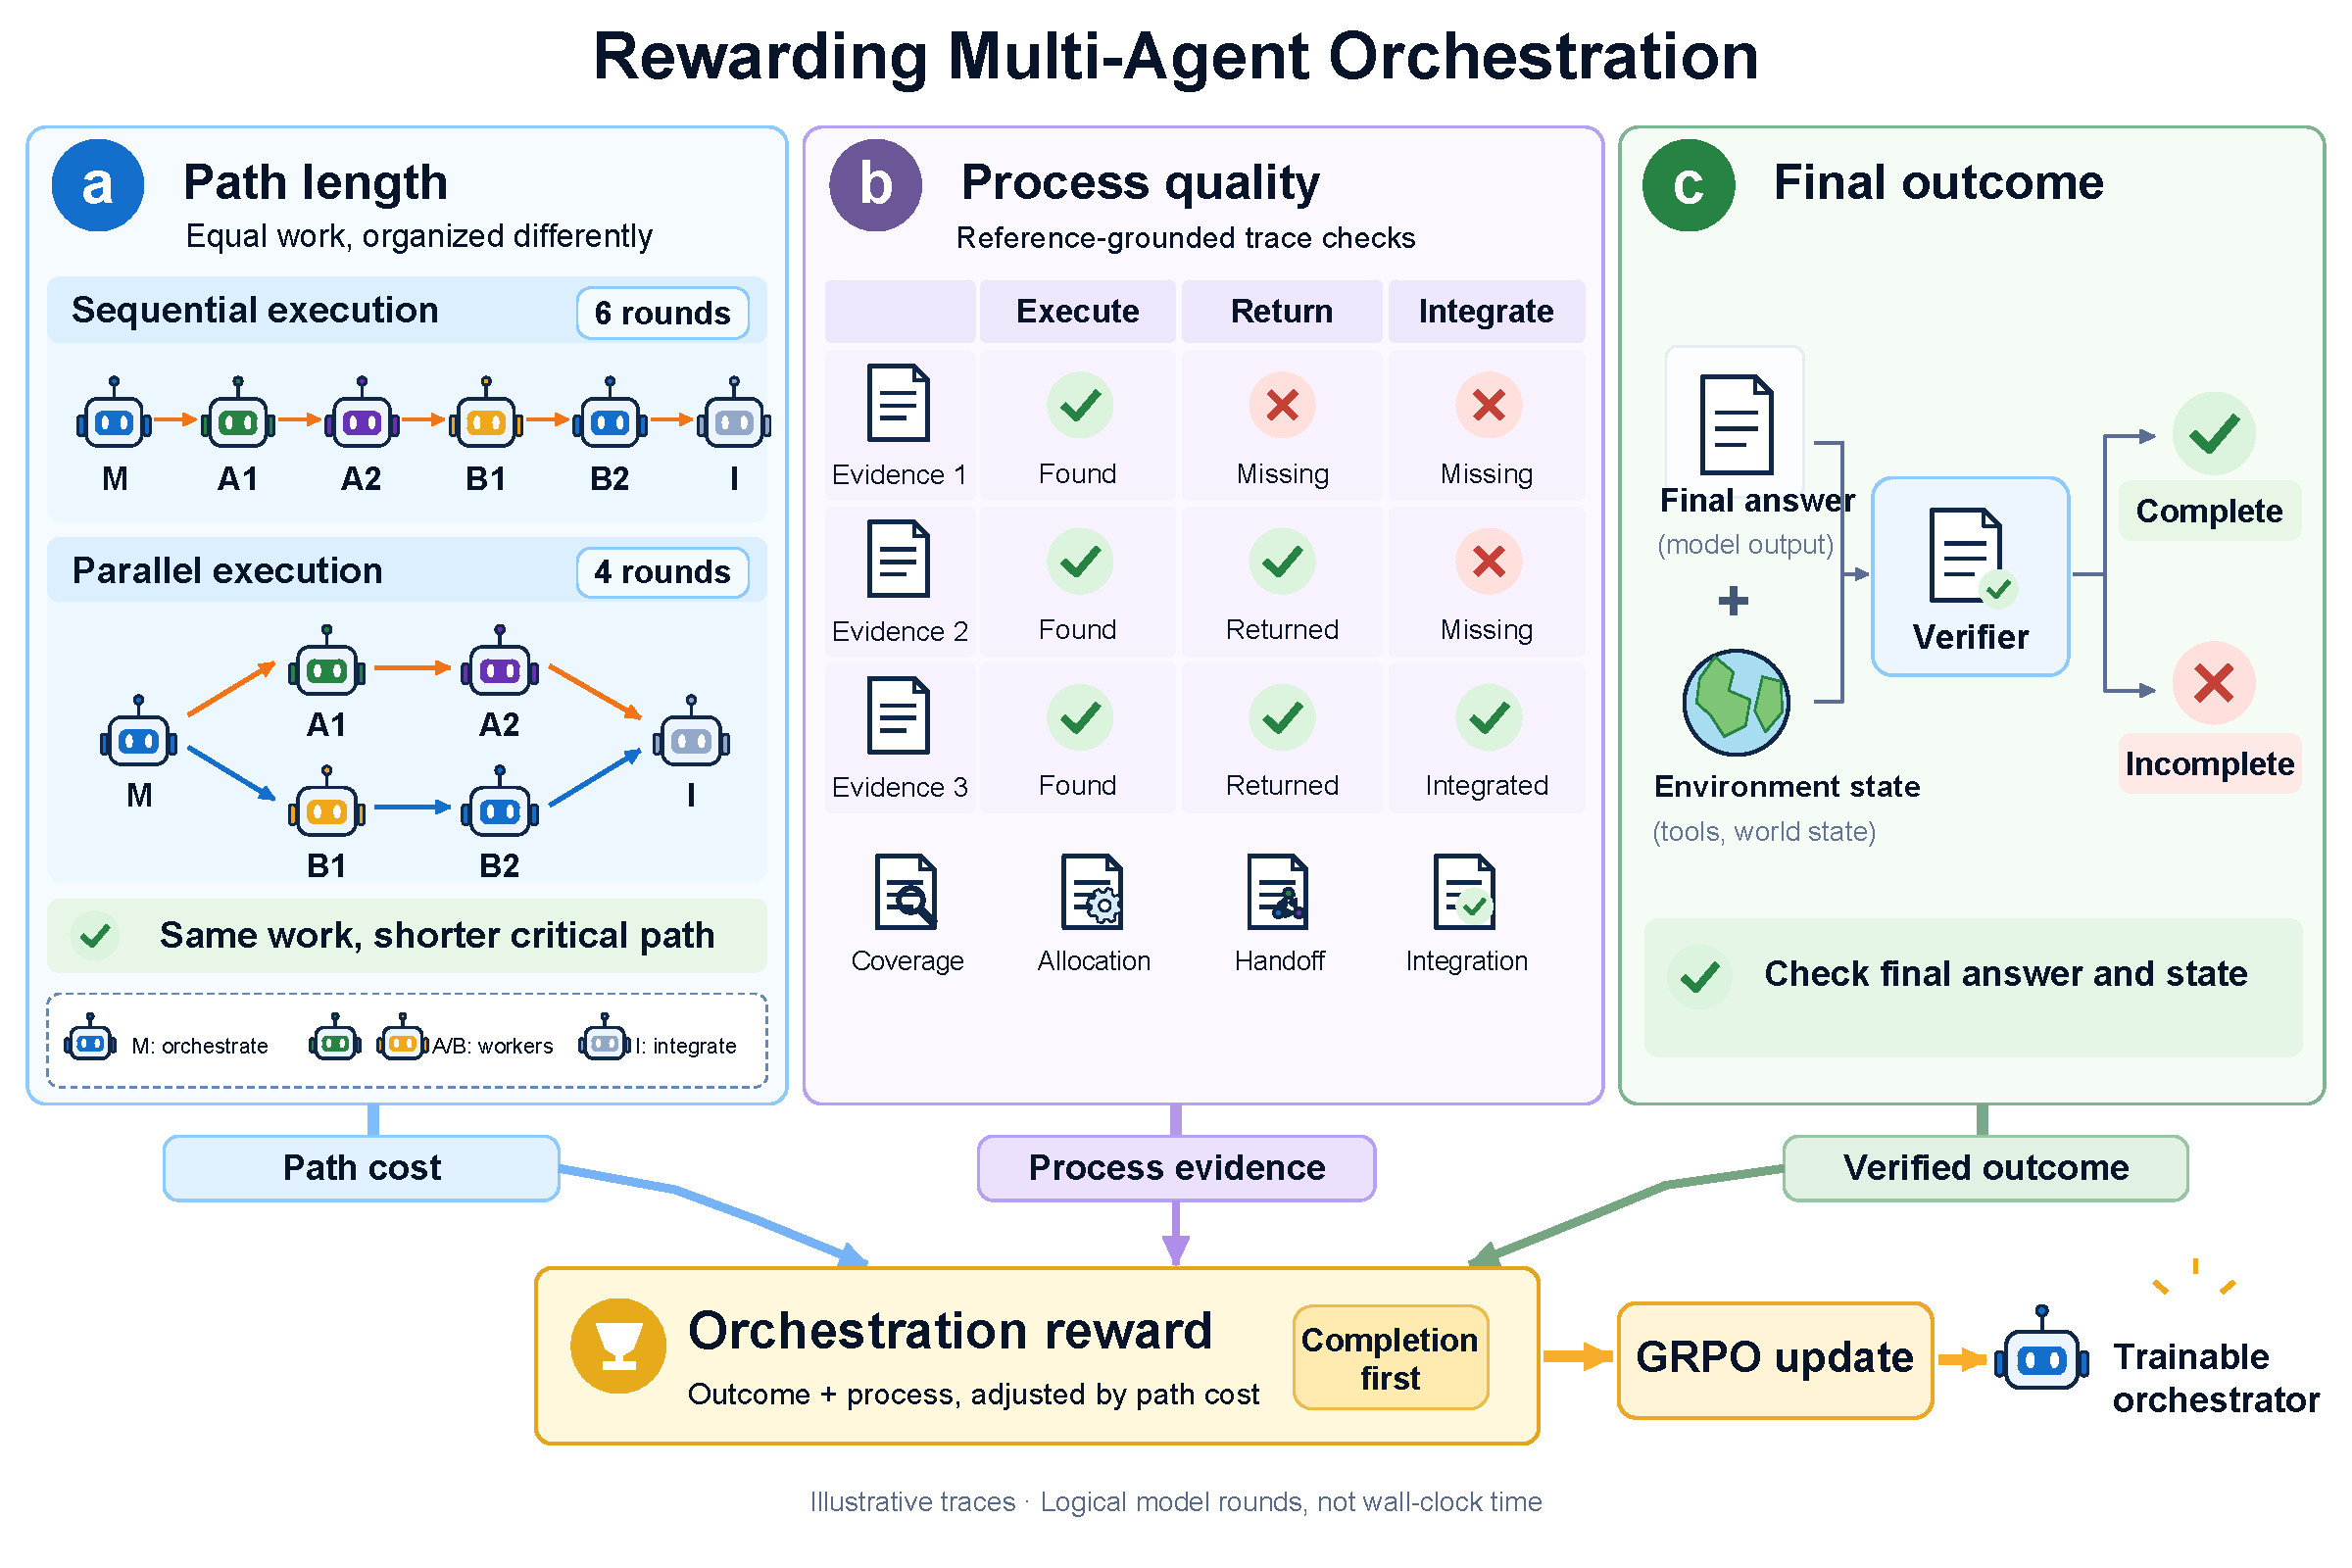
\includegraphics[width=\linewidth]{figures/figure4.pdf}
  \caption{Three sources of the orchestration reward. Equal work organized in parallel shortens the critical path (a), reference-grounded checks separate execution, return, and integration for every piece of evidence (b), and the verifier accepts a trajectory only when the final answer and the environment state both hold (c).}
  \label{fig:reward}
\end{figure}

\textbf{Schedule-aware Process Reward.}\quad
As shown in Figure~\ref{fig:reward}, the process term scores four properties of a team execution, namely the reference work completed, the requested answer present, the evidence returned by workers, and the independent work scheduled as independent,
\begin{equation}
f_{\mathrm{proc}}(\tau)=\alpha_{\mathrm{t}}f_{\mathrm{tool}}(\tau)+\alpha_{\mathrm{a}}f_{\mathrm{ans}}(\tau)+\alpha_{\mathrm{d}}f_{\mathrm{del}}(\tau)+\alpha_{\mathrm{s}}f_{\mathrm{sch}}(\tau),
\label{eq:proc}
\end{equation}
where every term lies in $[0,1]$ and the weights $\alpha$ are fixed once for all experiments (Table~\ref{tab:config}).
The tool term $f_{\mathrm{tool}}$ is the fraction of reference calls in $V$ matched once by a successful event with equivalent arguments and observation.
The answer term $f_{\mathrm{ans}}$ gives recall-oriented partial credit over the top-level fields of the answer, with a precision factor that removes any gain from padding the submission (Appendix~\ref{app:process}).
A team recovering most of the answer is thereby separated from one recovering none.
The delivery term $f_{\mathrm{del}}$ is the fraction of assigned subtasks whose worker return carries the required evidence, which measures the handoff a single agent never performs.
The schedule term is the part of the reward that no terminal verifier can express, and it reads the independence record produced by Eq.~\ref{eq:pi},
\begin{equation}
f_{\mathrm{sch}}(\tau)=(1-\delta_\tau)\cdot f_{\mathrm{int}}(\tau)\cdot\frac{|\Pi_\tau|}{|\Pi|},
\label{eq:sched}
\end{equation}
The leading ratio is the fraction of verified independent pairs that the team actually ran as independent, where $\Pi_\tau\subseteq\Pi$ contains the pairs assigned to two different workers under assignment intervals that do not depend on each other.
Two factors keep that ratio honest, since $\delta_\tau$ discounts assignments that repeat a covered subtask and $f_{\mathrm{int}}$ discounts branch results that never reach the final answer.
Eq.~\ref{eq:sched} is where synthesis and learning meet, as $\Pi$ exists only because composition proposed a branch and a reordered execution confirmed it.
A team is therefore credited for parallel work only on branches the environment has proven parallel, which is a judgement that terminal success cannot make.
A task whose reference contains no verified independent pair falls back to a conservative progress score, and Appendix~\ref{app:process} specifies that branch.

\textbf{Orchestrator-only Policy Optimization.}\quad
Partial progress requires enough weight to distinguish failing rollouts and little enough to never compete with a verified success.
The two terms are combined as
\begin{equation}
R(\tau)=f_{\mathrm{out}}(\tau)+\lambda\,f_{\mathrm{proc}}(\tau),\qquad \lambda=0.3,
\label{eq:reward}
\end{equation}
which gives a successful team at least $1$ and an unsuccessful team at most $\lambda$.
Process credit thereby separates failed rollouts without ever outweighing success.
For each task we sample $K$ team trajectories from independently reset environments and compute the group-relative advantage $A_i=(R_i-\bar{R})/(\mathrm{std}(R_1,\dots,R_K)+\epsilon)$ of the $i$-th trajectory.
The orchestrator is then updated with the clipped GRPO objective~\citep{shao2024deepseekmath}, written as
\begin{equation}
J(\theta)=\mathbb{E}\Bigl[\tfrac{1}{K}\textstyle\sum_{i=1}^{K}\tfrac{1}{|\mathcal{T}_i|}\sum_{t\in\mathcal{T}_i}\min\bigl(\rho_{it}(\theta)A_i,\ \mathrm{clip}(\rho_{it}(\theta),1-\epsilon_l,1+\epsilon_h)A_i\bigr)\Bigr],
\label{eq:grpo}
\end{equation}
where $\mathcal{T}_i$ contains only the tokens generated by the orchestrator and $\rho_{it}$ is the ratio between the current and the behavior policy on that token.
Worker generations and tool observations enter the context of the orchestrator and stay out of $\mathcal{T}_i$.
Since $\pi_\phi$ is never updated, every measured change comes from orchestration and not from worker quality.
